\documentclass{article}

\usepackage{amsmath}
\usepackage{hyperref}
\usepackage{dirtytalk}
\usepackage{tikz}
\usepackage{textcomp}
\usetikzlibrary{shapes,arrows, positioning}

% aquote environment
% from https://tex.stackexchange.com/questions/13756/quote-environment-with-reference-at-the-end-right

\def\signed #1{{\leavevmode\unskip\nobreak\hfil\penalty50\hskip2em
  \hbox{}\nobreak\hfil(#1)%
  \parfillskip=0pt \finalhyphendemerits=0 \endgraf}}
\newsavebox\mybox
\newenvironment{aquote}[1]
  {\savebox\mybox{#1}\begin{quote}}
  {\signed{\usebox\mybox}\end{quote}}

% end aquote environment

\title{GiG: A Decentralized Platform\\for the Gig Economy}
\author{Ishtar Eve}
\date{February 2019}
\begin{document}

\maketitle

\begin{abstract}
A decentralized application for the labor marketplace that connects employers with independent contractors is described. GiG, a system that works on the Cardano blockchain, is intended to reduce friction and to eliminate fees collected by employment agencies, recruiting platforms, and financial institutions. 

\paragraph{} The native currency of the system is the Gig Economy Token (GET). The algorithm used for its creation prevents speculative bubbles, and funds a Treasury System DAO (Decentralized Autonomous Organization), while guaranteeing scarcity. The DAO finances expenses for the ecosystem through proposals created and voted by the GiG community.

\paragraph{} GiG offers multiple tools that will give value to freelancers and employers, gaining the ability to interact without the need of trust, transacting on a peer to peer basis.

\paragraph{} Note: GiG is under construction. New versions of this paper will be updated periodically.

\end{abstract}

\newpage
\tableofcontents
\newpage

\section{Introduction}

The Intuit 2020 Report\cite{intuit-2020-report} cites, among many predictions, that the gig economy will be about 43\% of the workforce by 2020. Specifically, \say{work shifts from full-time to free agent employment}, \say{the Great Recession will continue accelerating the long-term trend toward a contingent workforce. Contingent workers – freelancers, temps, part-time workers, contractors and other specialists – are hired on a nonpermanent basis and don’t have full-time employment status.}. \say{Over the next decade, the number of contingent employees will increase worldwide. In the U.S. alone, contingent workers will exceedate 40 percent of the workforce by 2020.}. Finally, \say{over the next decade,
small businesses will develop their own collaborative networks of contingent workers, minimizing fixed labor costs and expanding the available talent pool}.

\paragraph{}The tendencies that these predictions suggest, are giving a heightened importance and value to systems that allow freelancers and employers to connect and interact.

\paragraph{}Another tendency that has been maniffesting lately, is decentralization. Thanks to the birth and development of blockchain technology, people engaging in all kinds of financial interactions have started to desintermediate middlemen, and use peer to peer platforms. 

\paragraph{} All around the world, there's lots of work that needs to be done, and many people who need to work. Unfortunately, the people who are willing to pay a certain amount of money for a certain work to be done, very often can't connect with the people who would be willing to do the work in exchange for such amount, and who would benefit from said laboral opportunity.

\subsection{Understanding the Gig Economy}
In a Gig Economy, temporary, flexible jobs are commonplace and companies tend towards hiring independent contractors and freelancers instead of full-time employees\cite{gig-economy-investopedia}. Let's crack down the details of this:

During most of the history, jobs tend to be stable for a lifetime, and often beyond a lifetime. For example, in the Middle Ages, a smith would often work during his whole life as a smith, and wouldn't change his employer during this time. Even more, the descendants of this smith would learn the craft from his parent, and would continue being smiths. This way, the job of being a smith spanned so long that it lasted even more than a lifetime. This happened because becoming decently productive required a lifetime of learning and a few secret tricks from your parents in order to be able to construct great results from the rudimentary tools available. This started to change with the Industrial Age. Strong, fast machines allowed to replicate a lifetime of performance in a few days, and the value shifted from being able to construct great merchadise to being able to command a machine to make great merchadise. As technology improved, inevitably the life-long jobs started to lose importance. Even more, some people started to specialize in creating technology faster, which made the improvement even faster, and the life-long jobs less valuable. This change shifted to high gear in the Information Age we currently live. Whereas in the Middle Ages a craftsman could only learn from the few people in his town that knew the craft, today, anyone with access to the Internet can learn from videos, papers and documents from the best specialists from all over the world. In the Information Age, whoever can read, digest and use the available information has a very valuable edge over the others in the whole world.

The other side of this valuable edge in the Information Age is that companies are interested in looking for this few specific people that already know and understand the market the company is trying to serve. And finally, the ability to reach these specialists accross the world using the Internet means that a company doesn't even have the need of having an office or even full-time employees in the same office or city.

All these factors make this labour market significantly different from traditional markets:

\begin{enumerate}
  \item Specialists can appear anywhere in the world, and companies are willing to hire them regardles of if they live in the same continent in the world or not.
  \item Dissemination and movement of information allows people from unexpected parts of the world to reach markets in other parts of the world.
  \item Competition becomes global. The cost of hiring specialists in a local market becomes less different because these specialists are now sought by companies from all over the world.
  \item Competition becomes global. The cost of being mediocre is now higher, because local companies may choose to hire strong remote specialists over mediocre local ones.
  \item The cost of running local operations in new locations is lower. Companies from other places of the world can hire local specialists to deliver specific actions in their city, without having to fly full-time employees to that city, or having to open and staff a local office.
  \item Discovery of the best specialist that can fullfill the job becomes the bottleneck. The market is now an information-discovery market. A company can run operations in a remote city in the world if it can manage to find and hire good freelancers to deliver that work locally. Freelancers looking for work have to figure out a way to be reached by remote companies looking for freelancers.
  \item With global specialists available for hire, hiring a full-time employee, and training him to become strong enough to compare with a specialist, is a losing battle. Not only is more expensive, it also takes more time, time that is used by the competition to get a hold of the market. Thus temporary, flexible jobs triump over hiring full-time employees.
  
  \item Here we should describe "why the blockchain". Then, we need a chapter describing the use of the GET token. And then, we can talk about the GET token creation.
\end{enumerate}

\newpage
\section{System Overview}

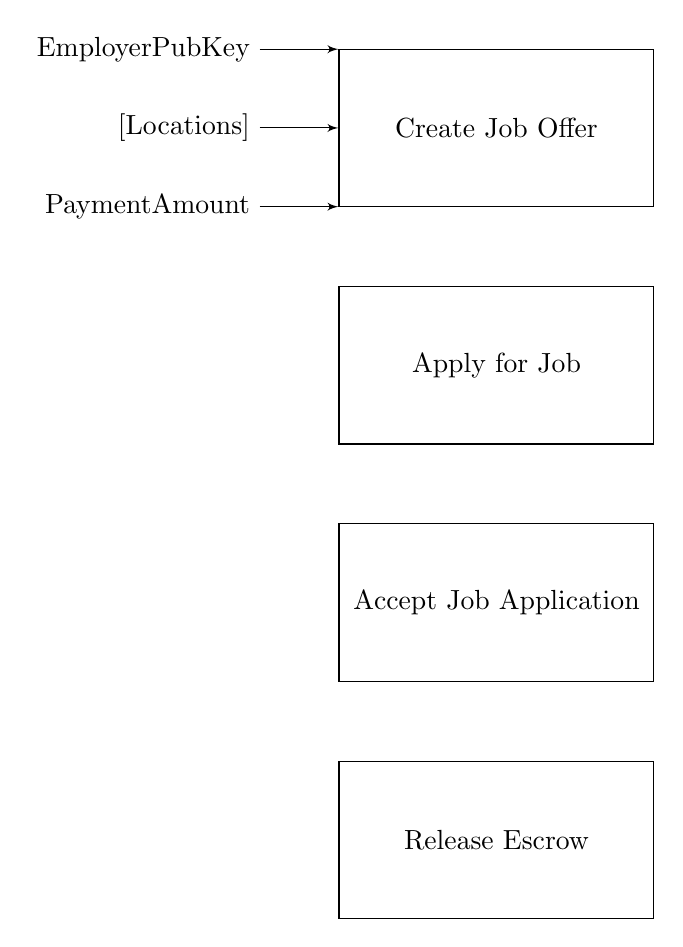
\begin{tikzpicture}[%
    %,node distance=30mm
    ,>=latex'
    ,block/.style = {%
        ,draw
        ,minimum height=20mm,minimum width=40mm
        ,align=center
        }
    ,every path/.style={->} 
    ]
\node (cjo) [block] {Create Job Offer};
%\coordinate[below right= 8mm and 8mm of cjo.east]  (joh);
\node (afj) [block, below= of cjo] {Apply for Job};
\node (aja) [block, below=of afj] {Accept Job Application};
\node (re) [block, below=of aja] {Release Escrow};


%\draw (cjo) to (joh);
%\draw[-latex'] (cjo.east |- joh) -- (joh) node[below = 20mm of cjo] {Job Offer Hash};
%\draw (joh) to (afj);
%\draw (afj) to (aja);

% Data for Apply for Job
\coordinate[above left = of cjo.west]   (a1);
\coordinate[below = of a1]              (a2);
\coordinate[below = of a2]              (a3);
\foreach \i [count=\xi from 1] in
{
    EmployerPubKey,
    [Locations],
    PaymentAmount
}
    \draw[-latex']  (a\xi) node[left] {\i} -- (a\xi-| cjo.west);

%\coordinate[below=of joh]  (joh);
%\coordinate[left = of afj.west]  (joh);
% \draw[-latex']  (joh) node[left] {Job Offer Hash} -- (cjo-| afj.west);
%\foreach \i [count=\xi from 1] in {Job Offer Hash}
%\draw[-latex'] (joh) -- (afj);
%\draw[-latex']  (a\xi) node[left] {\i} -- (a\xi-| cjo.west);
\end{tikzpicture}
\newpage

 
\section{Main Use Cases}
An application designed to connect employers and freelancers must offer basic use cases that allow completing the main type of transaction in the system: freelancer being able to work for an employer, and this freelancer getting paid by the employer when completing the work.

\subsection{Creating Job Offers}
An employer signs a job offer posting transaction with his Cardano private key. This transaction will always include an amount of get offered for the task, and a description of said task. The transaction might also include other information about the task, such as a location list, a expected schedule, and other instructions or information about the task.

This is implemented by posting a DataScript transaction to a Smart Contract that we decided to call the \emph{Job Board}. This initial transaction may have no ADA associated, and it's intended to broadcast to the community that a new job is available. It has to include enough information for the freelancers to decide if it's interesting to them, and this is implemented by using a DataScript with fields to describe the job being offered, and includes the public key of the employer.

The first iteration of the protocol contains just enough information to prove communication can be achieved, and may be extended later with fields of interest.

\begin{samepage}
\begin{verbatim}
data JobOffer = JobOffer
  { joDescription :: ByteString
  , joPayout      :: Int
  , joOfferer     :: PubKey
  }
  deriving (Show, Eq, Ord, Generic)
PlutusTx.makeLift ''JobOffer
\end{verbatim}
\end{samepage}

\subsection{Applying for Job Offers}


In order for a freelancer to find jobs, first he must be checking the place where employers post jobs: the Job Board. Thus, the first step for a freelancer is start listening for transactions in the Job Board address. As employers post new transactions there, the freelancers will be notified by their wallets of these operations. Then, the freelancers must be able to parse back the descriptions. The system uses the Plutus programming language for smart contracts, and this language, when compiled to the Plutus bytecode (known as CEK code), is not readable by human beings. In order for a freelancer to read and understand a job offer, we need to offer him a human-readable version of the posted job. This is done by means of the mechanism described in ``A pub-sub mechanism for Cardano and Plutus''\cite{pub-sub-paper}. Once this Plutus bytecode is parsed back to a standard machine representation, it's easy for the system to convert this machine representation into a user interface for the freelancer.

Now that the freelancer can understand what the job demands, he can apply to it. In this context, application means that the freelancer considers himself good enough to deliver the job required, but the employer may disagree. This is why further filtering before the job is done and the payment is delivered is needed. In this case, the freelancer posts his application to a different address, that we call the \emph{Job Application Board}. This address is derived automatically from the main Job Board address, hashing into it the specific details of the job.

The freelancer posts to this Job Application Board his public key, and possibly some relevant information. For the first iteration of the protocol, we have decided that the freelancer will only post his public key.

\begin{samepage}
\begin{verbatim}
data JobApplication = JobApplication
  { jaAcceptor    :: PubKey
  }
  deriving (Show, Eq, Generic)
PlutusTx.makeLift ''JobApplication
\end{verbatim}
\end{samepage}

\subsection{Accepting Applications by creating an Escrow}
At this point, both the employer and the freelancer share some common agreement (the job contract), and both parties have copies of the public keys of the other. They can now use standard asymmetric-cipher communication to further discuss the job terms and the ability of the freelancer to deliver the job. This is not covered by this paper, but it's relevant for the mechanism to be complete, and therefore will be addressed in further publications.

After the employer and the freelancer have reached an agreement, it is signed by the employer creating an escrow and locking the funds for payment. At this point, the freelancer can see the employer willingness to pay for the job by observing the escrow with the associated funds on the blockchain.

The underlying datatype in a DataScript that configures an escrow looks like:

\begin{samepage}
\begin{verbatim}
data EscrowSetup = EscrowSetup
  { esJobOffer        :: JobOffer
  , esJobApplication  :: JobApplication
  , esArbiter         :: PubKey
  }
  deriving (Show, Eq, Generic)
PlutusTx.makeLift ''EscrowSetup
\end{verbatim}
\end{samepage}

At this point, we have introduced another stakeholder without describing his role: the arbiter. The arbiter is a fundamental piece of the dispute resolution process that is described a few sections below.

\subsection{Escrow Release}
The freelancer now will proceed to deliver the work. When the employer agrees that the work has been delivered, he can release the funds in the escrow to the freelancer by posting a transaction to the escrow smart contract attaching his order to release as a RedeemerScript. This transaction is signed with the employer's private key, and assigns the funds to the freelancer's wallet.

\begin{samepage}
\begin{verbatim}
data EscrowResult
  = EscrowAcceptedByEmployer Signature
  ...
  deriving (Show, Eq, Generic)
PlutusTx.makeLift ''EscrowResult
\end{verbatim}
\end{samepage}


\subsection{Dispute Resolution}
Not every time the freelancer and the employer will agree on the outcome of the work delivered. When this happens, the employer may choose to not release the funds, which puts the situation in a stalemate, as the freelancer may not want to work more, and the employer has the funds locked in the smart contract.

To break this stalemate we introduce a third party: an arbiter. The arbiter has been agreed upon before the escrow creation, and his public key is now part of the escrow DataScript. The arbiter has power to release the funds to the freelancer, or back to the employer, but not to himself. It is expected for the arbiter to review any evidence provided by the employer and the employee, and release the escrow in favor of the actor whom he deems is in the right.

The escrow is released by the arbiter by posting a transaction to the escrow address with the result of his judgment (accept escrow to freelancer, or reject escrow back to employer), written as a RedeemerScript, setting the output of the transaction to the wallet of the freelancer or the wallet of the employer, and finally signing the transaction with his private key.

\begin{samepage}
\begin{verbatim}
data EscrowResult
  = EscrowAcceptedByEmployer Signature
  | EscrowAcceptedByArbiter Signature
  | EscrowRejectedByArbiter Signature
  deriving (Show, Eq, Generic)
PlutusTx.makeLift ''EscrowResult
\end{verbatim}
\end{samepage}

\section{Smart contracts}
Therefore, the system uses three main smart contracts: one for broadcasting the job, another for freelancers to apply to job offers, the final one for escrow and dispute resolution.

\subsection{Job Board Smart Contract}
The Job Board Smart Contract is somewhat simple, as it doesn't have to do advanced data processing and validation of transactions. Its main objective is forwarding information from the employer to the freelance, and back. In order to signal that a job is no longer available (for example, because it has been performed and is no longer needed), the employer is offered the option of closing it. This becomes the only validation this smart contract will do: whoever posts to the Job Board is the only one that can take it down.

The system uses the Watched Addresses abstraction provided by Plutus. This abstraction provides a way to specify which addresses (such as the Job Board and the Job Application Board) we want to observe, and the system will tell us non-complete transactions that are currently there. Because we use this system to read back job offers, we can take down a job offer by completing the transaction that posted the job offer, and thus making it disappear from everyone's Watched Addresses.

\begin{samepage}
\begin{verbatim}
jobBoard :: ValidatorScript
jobBoard = ValidatorScript ($$(Ledger.compileScript [||
  \(JobOffer {joOfferer}) () (t :: Validation.PendingTx) ->
    let
        Validation.PendingTx {
          pendingTxInputs=[_],
          pendingTxOutputs=[
            Validation.PendingTxOut {
              pendingTxOutData=Validation.PubKeyTxOut pubkey
            }
          ]
        } = t  -- It's fine if this fails matching,
               -- as it will cause the validator to error out
               -- and reject the transaction.

        inSignerIsSameAsOutSigner = $$(Validation.eqPubKey) pubkey joOfferer

    in
    if inSignerIsSameAsOutSigner
    then ()
    else $$(PlutusTx.error) ()
  ||]))
\end{verbatim}
\end{samepage}

The Job Board Smart Contract demands that whoever posted the job must take it down, and this is the only validation implemented in this contract. This allows the poster to notify the world when the job is available, and when it's no longer available, while preventing malicious third parties from closing the job contract without the employer's approval.

\subsection{Job Application Board Smart Contract}
Once a job has been published to the Job Board, we can derive a second address: the Job Application board address. This is done by using one of Plutus mechanisms that allow to use plain old currying/uncurrying to apply one of the parameters of a multi-parameter function and get as result a unique version of that function with that parameter applied.

\begin{samepage}
\begin{verbatim}
jobAcceptanceBoard :: ValidatorScript
jobAcceptanceBoard = ValidatorScript ($$(Ledger.compileScript [||
  \(_ :: JobOffer)
   (_ :: JobApplication)
   ()
   (_ :: Validation.PendingTx)
   ->
    -- TODO: Implement some validation here
    ()
  ||]))

jobAddress :: JobOffer -> Address
jobAddress jobOffer = Ledger.scriptAddress (ValidatorScript sc)
  where
    sc = (getValidator jobAcceptanceBoard) `applyScript` offerScript
    offerScript = Ledger.lifted jobOffer
\end{verbatim}
\end{samepage}

We derive the Job Acceptance Board address by applying the \verb|JobOffer| to the \verb|jobAcceptanceBoard| validator, which constructs a new validator specific to our Job. This assumes no jobs will ever be repeated, which is something that may have to change in the future.

The employer is expected to be listening on the corresponding Job Acceptance Board addresses for the jobs he has posted, with the intention of getting a feed of applicants to his job openings. The freelancers are expected to post their contact information as a transaction, with a \verb|JobApplication| \verb|DataScript| to the Job Acceptance Board, without associated payment. This way, they can communicate their interest in the job offer and forward contact information.

\subsection{Escrow Smart Contract}
The Escrow Smart Contract is significantly more complex than the Job Board and the Job Application Board Smart Contracts for two reasons:

\begin{itemize}
  \item The Escrow has funds that malicious actors may seek to steal.
  \item The Escrow may have to release these funds to different parties.
\end{itemize}

For this reason, the Escrow must have much tighter security and validation.

As usual, every Plutus Smart Contract is configured with a DataScript. In the Escrow DataScript we introduce the full job description (including the public key of the employer), as well as the description of the accepted freelance (including his public key), and the public key of the chosen arbiter.

\begin{samepage}
\begin{verbatim}
jobEscrowContract :: ValidatorScript
jobEscrowContract = ValidatorScript ($$(Ledger.compileScript [||
  \ (setup :: EscrowSetup)
    (result :: EscrowResult)
    (tx :: Validation.PendingTx)
    ->
    let EscrowSetup {
          esJobOffer=JobOffer {
            joOfferer=employerPubKey
          },
          esJobApplication=JobApplication {
            jaAcceptor=employeePubKey
          },
          esArbiter=arbiterPubKey
        } = setup
    in
		...
  ||]))
\end{verbatim}
\end{samepage}

The Escrow Smart Contract will now validate the actions that try to spend the escrow, and will check that the signer of the action is in position to execute the action, by checking the signatures of these actions.

\begin{samepage}
\begin{verbatim}
jobEscrowContract :: ValidatorScript
jobEscrowContract = ValidatorScript ($$(Ledger.compileScript [||
  \ (setup :: EscrowSetup)
    (result :: EscrowResult)
    (tx :: Validation.PendingTx)
    ->
		...
    let
      eqPubKey = $$(Validation.eqPubKey)
      signedBy' (Signature sig) (PubKey pk) = ...
      (&&) = $$(PlutusTx.and)
    in
    case result of
      EscrowAcceptedByEmployer sig ->
        if (signedBy' sig employerPubKey)
            && (eqPubKey destPubkey employeePubKey)
        then ()
        else $$(PlutusTx.error) ()

      EscrowAcceptedByArbiter sig ->
        if (signedBy' sig arbiterPubKey)
            && (eqPubKey destPubkey employeePubKey)
        then ()
        else $$(PlutusTx.error) ()

      EscrowRejectedByArbiter sig ->
        if (signedBy' sig arbiterPubKey)
            && (eqPubKey destPubkey employerPubKey)
        then ()
        else $$(PlutusTx.error) ()
  ||]))
\end{verbatim}
\end{samepage}

\section{The GET: Gig Economy Token}

(Write here why the GET shall exist)
(Is this section too soon to present the token? We haven't talked yet how we are going to solve the Gig Economy and we are already talking about a token)

\subsection{GET Token Creation}
GET tokens are created when ADA is received by the GET creation smart contract (GCSM).
The amount $\alpha$ of GET created and awarded to the ADA sender's wallet, will be an arbitrary constant $\phi$ (currently set to 1000), divided by the block height $\ell$, rounded up, starting from the first block since the GET creation smart contract gets published. That is,

\[ \alpha
  = \dfrac{\phi}{\ell}
\]

This policy has several effects:

\begin{enumerate}

  \item The cost of producing GET tokens via the smart contract will increase over time. 
  \item It provides an incentive to adopt the GiG Economy Token sooner than later. 
  \item The conversion rate provides a temporary price roof (in terms of ADA). In detail, if the market price climbs higher than the cost of creating GET, market actors will prefer producing GET via the smart contract rather than buying it in the market.
  \item Creating new tokens costs more over time, thus putting a positive price pressure on the existing tokens.
  \item Speculative pumps and dumps will be avoided, as the market price of buying GET will always be equal or lower to the cost of creating the token (by sending ADA to the GCSM). If there is no supply of GET in the market at a price equal or lower to the cost of creating GET, interested buyers would create them by sending ADA to the GCSM. 
  \item In the long term, creating GET through the GCSM will not be attractive, this means the GET supply has a theoretical hard cap.
  \item All the GET created by the GCSM will fund the DAO. So, if the market price pumps in a way that exceeds the cost of creating GET through the GCSM, there is an incentive to fund the DAO.
\end{enumerate}

\subsection{Treasury System and DAO}

All the ADA received by the GCSM is managed by a treasury system DAO based on the research made by IOHK for the Zendao \cite{zhangb2}. The objective of this treasury system is the funding and administration of the development of the GiG Economy Token platform.

A treasury system is a descentralized decision-making fund controlled by the community. It represents a mechanism to fund the development and mantainance of a project. It provides means for collaborative intelligence through democratic processes and vote delegation. 

Given the descentralized nature of the project, it is not coherent that it would get founding solely from an ICO or a founder's reward, this would put pressure on a central instution. In contrast, creating a Descentralized Autonomous Organization (DAO) to fund the project lets the stake holders of the GIG token decide how to use the funds that will power the plataform. 

Although a detailed description of the DAO's functionality can be found in the Zendao paper by IOHK, this are some of its features that are worth mentioning:

\begin{enumerate}

  \item Participating node's voting power will be proportional to the amount of coins in stake. 
  \item The treasury system will not link voters to their real identities.
  \item A vote can be represented as "Yes/No/Abstain".
  \item During each treasury period, a finite amount of proposals are elected by the stakers, this proposals will receive the funds from the DAO's treasury.
   
\end{enumerate}


\subsection{DAO funding}



\section{Prototype application}
At the time of writing this document, Plutus is not yet available in a testnet, and whoever want to try it have to use it through the Plutus Playground, or through the underlying emulator the Plutus Playground uses: the Mockchain.

\subsection{Beyond the Plutus Playground}
The Plutus Playground offers a nice and easy to use interface for interacting with the Mockchain, but it is severely limited, specially in the terms we are going to use.

\begin{itemize}
  \item First of all, the Plutus Playground offers us an interface we may or may not agree to use, but, in any case, is not the interface we expect from the system. We want the ability to use our own interface, in order to apply the UI/UX we consider adequate for the project.
  \item Second, the Plutus Playground doesn't allow us to do advanced manipulation of smart contracts, such as reading and parsing back DataScripts.
  \item Finally, the Plutus Playground doesn't have the ability to save files to a version control system that all modern software development workflow expects.
\end{itemize}

For these three reasons, we had to discard the Plutus Playground soon, and jump quickly to directly use the Mockchain in a prototype. This allowed us to understand deeply Plutus, and estimate real costs of integration with a real blockchain.

\subsection{Architectural considerations of the prototype}
The tech stack we chose for the prototype is a conservative choice given the most significant constraints in the system:

\begin{itemize}
  \item Plutus is written in Haskell, therefore the prime candidate programming language would be Haskell.
  \item We have some experience in web development, web development offers somewhat easy user interfaces with the usual entities (buttons, text, actions), and creating a web application allows us to offer the system easily over the Internet by just providing an URL. Therefore, constructing the prototype as a web application is our prime architectural decision.
  \item Although the blockchain is distributed in its nature, there is a \emph{centralized} concept behind it, being this concept the \emph{global agreement on a single chain}. We can simulate this global agreement locally without the problems that a distributed system creates by having a single Mockchain stored in a single machine. Although this defeats the distributed purpose of a real blockchain, we consider it good enough for a prototype phase, keeping in mind that a real blockchain with Plutus doesn't exist yet.
\end{itemize}

Following these three reasons, we have used as a base for our prototype a simple Yesod scaffolding with SQLite as database. Among the many web frameworks available, we chose this one because:

\begin{itemize}
  \item It is a web framework based in Haskell, therefore integrating Plutus should not be significantly hard.
  \item It is an \emph{opinionated} web framework. Opinionated web frameworks are the ones that have opinions: they have an opinion that you will use an specific architectural pattern, that you will use an specific template system, that you will use an specific data storage. In contrast, \emph{unopinionated} web frameworks feature an architecture where the developers have to connect whatever they need for the situation. In our experience, opinionated web frameworks work well for the large majority of projects, because their \emph{opinions} are conservative chosen, and a lot of integration effort has been already spent making their opinions fit nicely. Therefore, we chose Yesod in the Haskell world, because it is the opinionated web framework that mostly resembled the \emph{King of web frameworks}: Ruby on Rails.
  \item It is well supported by the community. This is important, as it will save time because there will be available plugins for most situations, and books, forums and blogs to help unblock the development team when they need it.
\end{itemize}

\subsection{Design approach of the prototype}
Now that we decided to use a web application, we can start to consider what this means in terms of it being a frontend for Plutus and the Mochckain:

\begin{itemize}
  \item We are going to store a single Mockchain in memory, and use it as our datastore.
  \item Actions performed by the different stakeholders of the system will be performed against this single in-memory Mockchain, usually by adding new blocks to it.
  \item We should try to use only the methods and operations that the Wallet API provides, as any other operation is not expected to be available on the real blockchain.
  \item If we have to use operations not provided by the Wallet API, we have to be careful to ensure these operations are plausible and somewhat expected to be available later. In any case, we can't do operations that break the constraints of the blockchain, such as rewriting blocks.
\end{itemize}

These constraints have proven to be a reasonable challenge, and have pushed our learning on how to construct distributed apps significantly. The only constraint we have broke regularly is the ability to rewrite the blockchain. By virtue of storing the Mockchain in memory, every time we restarted the system it forgot its history and restarted in a clean state. This has proven very useful for testing and validating ideas, and is expected on usual development workflows, but it's also something to keep in mind, as doing it in production systems is expected to be practically impossible.

\subsection{Lessons learnt from the prototype}
In our opinion, the usage of a web framework has paid significantly, as it provided a simple but powerful way to explore the user interfaces around Smart Contracts. We had to figure out when we have to offer different buttons for different actions, guided by the available information on the blockchain. This also lead us to interesting information distribution issues, that eventually lead to the discovery of unlifting and the Plutus Pub-Sub pattern\cite{pub-sub-paper}.

Ironically, the \emph{opinion} of using a SQLite database has not been used, as we focused on using the blockchain as our distributed store of data. Storing data in the blockchain is expected to be expensive\cite{transaction-fees}, so we can't truly discard the option of using an external and cheaper data storage.


\section{Architecture of the GiG Economy dApp}
The protoype serves as an effective way to learn and understand Cardano and Plutus, and direct that learning into the objectives we want to achieve. But it cannot be considered the final application because the constraints of the final application are significantly different to the constraints of the prototype.

\subsection{Architectural limitations of the prototype}

In order to construct the prototype quickly, we have paid little attention to many significant flaws in the current system:

\begin{itemize}
  \item There is no testnet with Plutus, which means we had to construct a prototype on top of the Plutus emulator, not on top of a real blockchain.
  \item There is an expectation of using a wallet to interact with the blockchain, because wallets store keypairs and deal with the blockchain in a great way, and it would be inadequate to not reuse all that research around connecting safely with the blockchain that has been done.
  \item It is not expected that end users will have to run web servers.
\end{itemize}

There are also more constraints that we haven't addressed in the prototype, but that will be significant when constructing the dApp:

\begin{itemize}
  \item User profiles, probably including photos and other data intensive entities will have to be stored somewhere for employers and freelancers to review. Storing lots of data in the blockchain is not viable because of transaction costs, so we need a different mechanism to solve this problem.
  \item Communication between employers and freelancers after the freelancer has applied to a job is not discussed. We assume that the freelancers and the employers will \emph{magically} use their public keys to reach an agreement. This has to be addressed in the dApp in order to be able to reach a significant group of people.
  \item We have introduced arbiters without a way to find them, and figure if they are good for dispute resolution. There is a gap waiting to be filled related to how a freelancer and an employer will reach an agreement on which arbiter is going to be called to resolve the escrow.
  \item Arbiters are expected to review all the evidence related to an escrow before deciding who is in the right. The prototype doesn't address how this evidence is going to be collected, stored, and delivered to the arbiter so that she can do her job.
  \item There is an expectation of rating the interaction, and each party having a rating in the system, because people are more willing to start interactions with people that have good reputation. We haven't addressed neither any kind of reputation in the prototype, nor how could it be gathered, stored and displayed.
  \item The real blockchain has transaction costs and fees that must be paid by someone for the transactions to be accepted. The prototype doesn't have such requirements, and therefore we have assumed that transaction costs are negligible. The dApp will have to consider, calculate, display and pay these transaction costs unless we can truly prove that they are negligible.
  \item Modern applications have created an expectation of instant communication that we haven't implemented in the prototype. For example, it is expected that the employer is somehow notified when a freelancer applies to a job. This will require creating a system that is able to react in a timely fashion to events that happen in the blockchain, and trigger actions outside the blockchain.
  \item We know the smart contracts we offer here are adequate for a prototype phase, and we expect to improve them over time. But there is no way in place to be able to replace a smart contract with an improved one, and this will require architecture considerations that we have not addressed yet.
  \item The prototype uses ADA for payments, but, for the project to be continuously funded, improved and guided, a cornerstone consists on using GET instead of ADA. There are lots of questions on how to implement, pay, vote and cover transaction fees using GET. The prototype has not addressed any of those questions, and the dApp will have to address them.
\end{itemize}

These changes mean the GiG Economy dApp will have to be significantly rearchitected around a wallet, and further research must be done in order to fill all the communication gaps currently present in the prototype, such as freelancer-employer communication, or freelancer-arbitrer communication.

\subsection{Architectural approach for the dApp}

For the dApp to be successful, it must offer:

\begin{itemize}
  \item An easy to use and effective way for users to interact with eachothers in the GiG Economy.
  \item An easy to use way for users to interact with the blockchain.
  \item An effective way to be discovered by new users.
  \item A compelling reason for veteran users to continue use it.
  \item A significant edge over currently-available solutions for users to decide to leave their current systems in favour of the GiG Economy dApp.
\end{itemize}

We will explore the solution space looking for hints of architectural design that allows us to cover these reasons.

\subsubsection{The application platform}

\begin{aquote}{the Daedalus website\cite{daedalus-website}}
Daedalus is a highly secure wallet for the Ada cryptocurrency. Download and install it so you can use it to safely store your Ada. Daedalus will add more cryptocurrencies and be developed over time along with Cardano, to become a universal wallet, blockchain application platform and an app store.
\end{aquote}


The Daedalus Wallet offers a good hint on how we can construct the GiG Economy dApp. It will offer in the future an app store and blockchain application platform, and it seems the GiG Economy dApp will have the most reach if it can use the provided blockchain application platform for running, and the app store for discovery and distribution. With good support from a known wallet, we can cover the requirements of using the blockchain easily, and being easy to find and install by new users.

There is a second wallet in the ecosystem called Yoroi. Yoroi aims to be a secure, fast and simple lightweight wallet\cite{yoroi-website}. We don't expect this wallet to offer a blockchain application platform, or an app store.

Therefore, there are two main types of wallets available in the Cardano blockchain. But the expected complexity of the GiG Economy dApp suggests that only \emph{heavyweight} wallets that offer a blockchain application platform may be viable for our purposes.

\subsubsection{Broadcasting and responding requirements}

There must be a way for employers to post job offers, and for freelancers to check the offers and apply to them. It may not be viable for the platform to store the complete job offer in the blockchain, as it may include lots of data and incur in significant transaction costs. For the same reason, it may not be viable for the platform to put in the blockchain a full application with the full profile of the freelancer. This means we need to look for alternative ways to store this information.

All the transactions that are posted to the blockchain become public. So there is another concern related to storing freelancer profiles (or references to profiles) in the blockchain. The profile may include sensitive information, and freelancers may not want to expose such information to everyone. On top of that, there are laws and regulations that affect how we can store and retrieve such sensitive information.

\subsubsection{Communication requirements}

There must be a way for employers, freelancers and arbiters to communicate with each other. This poses an initial challenge, as people may not want to reveal much of their contact information. This is very relevant, for example, for arbiters. If a malicious party discovers enough contact information of an arbiter (name, address, friends, family), he could use this information to coerce the arbiter into chosing an specific outcome regardless of evidence provided.

So we need to support a gradual level of contact information to be revealed, and we need to ensure this contact information is revealed only to the right parties.

\subsubsection{Market expansion requirements}

As the GiG Economy Platform expands, a way to discriminate jobs depending on circumstances is expected to be required. We may want to broadcast local jobs only to freelancers in the world that are in a situation to deliver them at the required location. This means we will have to investigate and implement a mechanism for specifying the outreach of a job, in order for freelancers to receive only jobs that may be relevant to them, and for employers to receive applications from freelancers that are in a good position to deliver the work.

This requirement also means we have to be careful when designing the smart contracts, so that we can configure them to have this calculated reach, and, at the same time, are able to withstand global actions and usage. This is specially important for the Gig Economy Token, as it is expected that the token is fungible (I/E every token is equal to any other token), and therefore is prime candidate for having a single smart contract to be aplied to every user of the system.

\subsubsection{Continuity requirements}

The GiG Economy Platform is expected to expand, change and evolve over time. Because it is intended to be a distributed platform, there can't be a single person or group of people that will govern it, as this group of people can be a weak point of the whole platform, and defeats the point of having a distributed application.

For this reason, we envision the Gig Economy Token as a mechanism for voting and administering the future of the platform, by constructing a Decentralized Autonomous Organization. The dApp must offer the mechanisms needed for people to fund and participate in this DAO.

As the platform evolves, it is expected that the Smart Contracts used by the platform will change. For the DAO to construct the next evolution of the platform, there must be a way to retire old contracts and replace them with new contracts, as well as ways for rejecting contracts for being obsolete or with known vulnerabilities. Inevitably, this leads to requiring some kind of listing of approved and rejected smart contracts, and the DAO must have the ability to update this listing.

\subsection{Architectural vision}

Considering these requirements, we can start drafting the architecture of the platform.

\begin{figure}[h]
  \centering{
    \large
    \resizebox{\textwidth}{!}{% Graphic for TeX using PGF
% Title: /Users/jcasas/projects/gig-economy-paper/diagrams/arch.dia
% Creator: Dia v0.97.2
% CreationDate: Fri Mar 22 16:56:32 2019
% For: jcasas
% \usepackage{tikz}
% The following commands are not supported in PSTricks at present
% We define them conditionally, so when they are implemented,
% this pgf file will use them.
\ifx\du\undefined
  \newlength{\du}
\fi
\setlength{\du}{15\unitlength}
\begin{tikzpicture}
\pgftransformxscale{1.000000}
\pgftransformyscale{-1.000000}
\definecolor{dialinecolor}{rgb}{0.000000, 0.000000, 0.000000}
\pgfsetstrokecolor{dialinecolor}
\definecolor{dialinecolor}{rgb}{1.000000, 1.000000, 1.000000}
\pgfsetfillcolor{dialinecolor}
\pgfsetlinewidth{0.100000\du}
\pgfsetdash{}{0pt}
\definecolor{dialinecolor}{rgb}{1.000000, 1.000000, 1.000000}
\pgfsetfillcolor{dialinecolor}
\fill (38.750000\du,4.000000\du)--(39.250000\du,3.500000\du)--(46.450000\du,3.500000\du)--(46.450000\du,18.500000\du)--(45.950000\du,19.000000\du)--(38.750000\du,19.000000\du)--(38.750000\du,4.000000\du)--cycle;
\definecolor{dialinecolor}{rgb}{0.000000, 0.000000, 0.000000}
\pgfsetstrokecolor{dialinecolor}
\draw (38.750000\du,4.000000\du)--(39.250000\du,3.500000\du)--(46.450000\du,3.500000\du)--(46.450000\du,18.500000\du)--(45.950000\du,19.000000\du)--(38.750000\du,19.000000\du)--(38.750000\du,4.000000\du)--cycle;
\definecolor{dialinecolor}{rgb}{0.000000, 0.000000, 0.000000}
\pgfsetstrokecolor{dialinecolor}
\draw (38.750000\du,4.000000\du)--(45.950000\du,4.000000\du);
\definecolor{dialinecolor}{rgb}{0.000000, 0.000000, 0.000000}
\pgfsetstrokecolor{dialinecolor}
\draw (45.950000\du,4.000000\du)--(46.450000\du,3.500000\du);
\definecolor{dialinecolor}{rgb}{0.000000, 0.000000, 0.000000}
\pgfsetstrokecolor{dialinecolor}
\draw (45.950000\du,4.000000\du)--(45.950000\du,19.000000\du);
% setfont left to latex
\definecolor{dialinecolor}{rgb}{0.000000, 0.000000, 0.000000}
\pgfsetstrokecolor{dialinecolor}
\node[anchor=west] at (39.250000\du,5.142500\du){};
\pgfsetlinewidth{0.050000\du}
\definecolor{dialinecolor}{rgb}{0.000000, 0.000000, 0.000000}
\pgfsetstrokecolor{dialinecolor}
\draw (39.250000\du,5.277500\du)--(39.250000\du,5.277500\du);
% setfont left to latex
\definecolor{dialinecolor}{rgb}{0.000000, 0.000000, 0.000000}
\pgfsetstrokecolor{dialinecolor}
\node at (42.350000\du,11.753750\du){Blockchain};
\pgfsetlinewidth{0.100000\du}
\pgfsetdash{}{0pt}
\definecolor{dialinecolor}{rgb}{1.000000, 1.000000, 1.000000}
\pgfsetfillcolor{dialinecolor}
\fill (14.500000\du,3.900000\du)--(15.000000\du,3.400000\du)--(34.400000\du,3.400000\du)--(34.400000\du,18.550000\du)--(33.900000\du,19.050000\du)--(14.500000\du,19.050000\du)--(14.500000\du,3.900000\du)--cycle;
\definecolor{dialinecolor}{rgb}{0.000000, 0.000000, 0.000000}
\pgfsetstrokecolor{dialinecolor}
\draw (14.500000\du,3.900000\du)--(15.000000\du,3.400000\du)--(34.400000\du,3.400000\du)--(34.400000\du,18.550000\du)--(33.900000\du,19.050000\du)--(14.500000\du,19.050000\du)--(14.500000\du,3.900000\du)--cycle;
\definecolor{dialinecolor}{rgb}{0.000000, 0.000000, 0.000000}
\pgfsetstrokecolor{dialinecolor}
\draw (14.500000\du,3.900000\du)--(33.900000\du,3.900000\du);
\definecolor{dialinecolor}{rgb}{0.000000, 0.000000, 0.000000}
\pgfsetstrokecolor{dialinecolor}
\draw (33.900000\du,3.900000\du)--(34.400000\du,3.400000\du);
\definecolor{dialinecolor}{rgb}{0.000000, 0.000000, 0.000000}
\pgfsetstrokecolor{dialinecolor}
\draw (33.900000\du,3.900000\du)--(33.900000\du,19.050000\du);
% setfont left to latex
\definecolor{dialinecolor}{rgb}{0.000000, 0.000000, 0.000000}
\pgfsetstrokecolor{dialinecolor}
\node[anchor=west] at (15.000000\du,5.042500\du){};
\pgfsetlinewidth{0.050000\du}
\definecolor{dialinecolor}{rgb}{0.000000, 0.000000, 0.000000}
\pgfsetstrokecolor{dialinecolor}
\draw (15.000000\du,5.177500\du)--(15.000000\du,5.177500\du);
\pgfsetlinewidth{0.100000\du}
\pgfsetdash{}{0pt}
\definecolor{dialinecolor}{rgb}{1.000000, 1.000000, 1.000000}
\pgfsetfillcolor{dialinecolor}
\fill (15.900000\du,12.550000\du)--(16.400000\du,12.050000\du)--(32.500000\du,12.050000\du)--(32.500000\du,17.700000\du)--(32.000000\du,18.200000\du)--(15.900000\du,18.200000\du)--(15.900000\du,12.550000\du)--cycle;
\definecolor{dialinecolor}{rgb}{0.000000, 0.000000, 0.000000}
\pgfsetstrokecolor{dialinecolor}
\draw (15.900000\du,12.550000\du)--(16.400000\du,12.050000\du)--(32.500000\du,12.050000\du)--(32.500000\du,17.700000\du)--(32.000000\du,18.200000\du)--(15.900000\du,18.200000\du)--(15.900000\du,12.550000\du)--cycle;
\definecolor{dialinecolor}{rgb}{0.000000, 0.000000, 0.000000}
\pgfsetstrokecolor{dialinecolor}
\draw (15.900000\du,12.550000\du)--(32.000000\du,12.550000\du);
\definecolor{dialinecolor}{rgb}{0.000000, 0.000000, 0.000000}
\pgfsetstrokecolor{dialinecolor}
\draw (32.000000\du,12.550000\du)--(32.500000\du,12.050000\du);
\definecolor{dialinecolor}{rgb}{0.000000, 0.000000, 0.000000}
\pgfsetstrokecolor{dialinecolor}
\draw (32.000000\du,12.550000\du)--(32.000000\du,18.200000\du);
% setfont left to latex
\definecolor{dialinecolor}{rgb}{0.000000, 0.000000, 0.000000}
\pgfsetstrokecolor{dialinecolor}
\node[anchor=west] at (16.400000\du,13.692500\du){};
\pgfsetlinewidth{0.050000\du}
\definecolor{dialinecolor}{rgb}{0.000000, 0.000000, 0.000000}
\pgfsetstrokecolor{dialinecolor}
\draw (16.400000\du,13.827500\du)--(16.400000\du,13.827500\du);
\pgfsetlinewidth{0.100000\du}
\pgfsetdash{}{0pt}
\pgfsetdash{}{0pt}
\pgfsetbuttcap
\pgfsetmiterjoin
\pgfsetlinewidth{0.100000\du}
\pgfsetbuttcap
\pgfsetmiterjoin
\pgfsetdash{}{0pt}
\definecolor{dialinecolor}{rgb}{1.000000, 1.000000, 1.000000}
\pgfsetfillcolor{dialinecolor}
\pgfpathmoveto{\pgfpoint{14.765712\du}{24.094242\du}}
\pgfpathcurveto{\pgfpoint{13.756869\du}{24.068024\du}}{\pgfpoint{11.800328\du}{24.618601\du}}{\pgfpoint{12.075467\du}{25.798409\du}}
\pgfpathcurveto{\pgfpoint{12.350603\du}{26.978216\du}}{\pgfpoint{13.665156\du}{27.240385\du}}{\pgfpoint{14.215434\du}{26.899562\du}}
\pgfpathcurveto{\pgfpoint{14.765712\du}{26.558729\du}}{\pgfpoint{13.359446\du}{28.551282\du}}{\pgfpoint{16.049694\du}{29.075641\du}}
\pgfpathcurveto{\pgfpoint{18.739917\du}{29.600000\du}}{\pgfpoint{20.115613\du}{28.761026\du}}{\pgfpoint{19.718189\du}{28.158013\du}}
\pgfpathcurveto{\pgfpoint{19.320766\du}{27.555000\du}}{\pgfpoint{22.072157\du}{29.573782\du}}{\pgfpoint{23.356139\du}{28.420193\du}}
\pgfpathcurveto{\pgfpoint{24.640121\du}{27.266603\du}}{\pgfpoint{22.041586\du}{26.165460\du}}{\pgfpoint{22.591864\du}{26.322767\du}}
\pgfpathcurveto{\pgfpoint{23.142142\du}{26.480075\du}}{\pgfpoint{24.823547\du}{26.270332\du}}{\pgfpoint{24.273269\du}{24.303986\du}}
\pgfpathcurveto{\pgfpoint{23.722991\du}{22.337640\du}}{\pgfpoint{18.770488\du}{23.858281\du}}{\pgfpoint{19.320766\du}{23.569883\du}}
\pgfpathcurveto{\pgfpoint{19.871044\du}{23.281486\du}}{\pgfpoint{18.495349\du}{21.839496\du}}{\pgfpoint{16.783398\du}{22.127894\du}}
\pgfpathcurveto{\pgfpoint{15.071422\du}{22.416294\du}}{\pgfpoint{14.949994\du}{22.939630\du}}{\pgfpoint{14.766568\du}{24.093220\du}}
\pgfpathlineto{\pgfpoint{14.765712\du}{24.094242\du}}
\pgfusepath{fill}
\definecolor{dialinecolor}{rgb}{0.000000, 0.000000, 0.000000}
\pgfsetstrokecolor{dialinecolor}
\pgfpathmoveto{\pgfpoint{14.765712\du}{24.094242\du}}
\pgfpathcurveto{\pgfpoint{13.756869\du}{24.068024\du}}{\pgfpoint{11.800328\du}{24.618601\du}}{\pgfpoint{12.075467\du}{25.798409\du}}
\pgfpathcurveto{\pgfpoint{12.350603\du}{26.978216\du}}{\pgfpoint{13.665156\du}{27.240385\du}}{\pgfpoint{14.215434\du}{26.899562\du}}
\pgfpathcurveto{\pgfpoint{14.765712\du}{26.558729\du}}{\pgfpoint{13.359446\du}{28.551282\du}}{\pgfpoint{16.049694\du}{29.075641\du}}
\pgfpathcurveto{\pgfpoint{18.739917\du}{29.600000\du}}{\pgfpoint{20.115613\du}{28.761026\du}}{\pgfpoint{19.718189\du}{28.158013\du}}
\pgfpathcurveto{\pgfpoint{19.320766\du}{27.555000\du}}{\pgfpoint{22.072157\du}{29.573782\du}}{\pgfpoint{23.356139\du}{28.420193\du}}
\pgfpathcurveto{\pgfpoint{24.640121\du}{27.266603\du}}{\pgfpoint{22.041586\du}{26.165460\du}}{\pgfpoint{22.591864\du}{26.322767\du}}
\pgfpathcurveto{\pgfpoint{23.142142\du}{26.480075\du}}{\pgfpoint{24.823547\du}{26.270332\du}}{\pgfpoint{24.273269\du}{24.303986\du}}
\pgfpathcurveto{\pgfpoint{23.722991\du}{22.337640\du}}{\pgfpoint{18.770488\du}{23.858281\du}}{\pgfpoint{19.320766\du}{23.569883\du}}
\pgfpathcurveto{\pgfpoint{19.871044\du}{23.281486\du}}{\pgfpoint{18.495349\du}{21.839496\du}}{\pgfpoint{16.783398\du}{22.127894\du}}
\pgfpathcurveto{\pgfpoint{15.071422\du}{22.416294\du}}{\pgfpoint{14.949994\du}{22.939630\du}}{\pgfpoint{14.766568\du}{24.093220\du}}
\pgfpathlineto{\pgfpoint{14.765712\du}{24.094242\du}}
\pgfusepath{stroke}
% setfont left to latex
\definecolor{dialinecolor}{rgb}{0.000000, 0.000000, 0.000000}
\pgfsetstrokecolor{dialinecolor}
\node at (18.661044\du,26.106549\du){Large Object Storage};
\pgfsetlinewidth{0.100000\du}
\pgfsetdash{}{0pt}
\pgfsetdash{}{0pt}
\pgfsetbuttcap
\pgfsetmiterjoin
\pgfsetlinewidth{0.100000\du}
\pgfsetbuttcap
\pgfsetmiterjoin
\pgfsetdash{}{0pt}
\definecolor{dialinecolor}{rgb}{1.000000, 1.000000, 1.000000}
\pgfsetfillcolor{dialinecolor}
\pgfpathmoveto{\pgfpoint{27.407549\du}{24.143903\du}}
\pgfpathcurveto{\pgfpoint{26.659121\du}{24.122922\du}}{\pgfpoint{25.207626\du}{24.563532\du}}{\pgfpoint{25.411743\du}{25.507698\du}}
\pgfpathcurveto{\pgfpoint{25.615857\du}{26.451863\du}}{\pgfpoint{26.591082\du}{26.661669\du}}{\pgfpoint{26.999315\du}{26.388919\du}}
\pgfpathcurveto{\pgfpoint{27.407549\du}{26.116160\du}}{\pgfpoint{26.364285\du}{27.710742\du}}{\pgfpoint{28.360094\du}{28.130371\du}}
\pgfpathcurveto{\pgfpoint{30.355884\du}{28.550000\du}}{\pgfpoint{31.376468\du}{27.878594\du}}{\pgfpoint{31.081633\du}{27.396020\du}}
\pgfpathcurveto{\pgfpoint{30.786797\du}{26.913447\du}}{\pgfpoint{32.827965\du}{28.529019\du}}{\pgfpoint{33.780510\du}{27.605835\du}}
\pgfpathcurveto{\pgfpoint{34.733055\du}{26.682651\du}}{\pgfpoint{32.805285\du}{25.801438\du}}{\pgfpoint{33.213519\du}{25.927327\du}}
\pgfpathcurveto{\pgfpoint{33.621752\du}{26.053216\du}}{\pgfpoint{34.869133\du}{25.885364\du}}{\pgfpoint{34.460899\du}{24.311755\du}}
\pgfpathcurveto{\pgfpoint{34.052666\du}{22.738146\du}}{\pgfpoint{30.378564\du}{23.955070\du}}{\pgfpoint{30.786797\du}{23.724274\du}}
\pgfpathcurveto{\pgfpoint{31.195031\du}{23.493478\du}}{\pgfpoint{30.174447\du}{22.339496\du}}{\pgfpoint{28.904405\du}{22.570292\du}}
\pgfpathcurveto{\pgfpoint{27.634345\du}{22.801090\du}}{\pgfpoint{27.544262\du}{23.219901\du}}{\pgfpoint{27.408184\du}{24.143085\du}}
\pgfpathlineto{\pgfpoint{27.407549\du}{24.143903\du}}
\pgfusepath{fill}
\definecolor{dialinecolor}{rgb}{0.000000, 0.000000, 0.000000}
\pgfsetstrokecolor{dialinecolor}
\pgfpathmoveto{\pgfpoint{27.407549\du}{24.143903\du}}
\pgfpathcurveto{\pgfpoint{26.659121\du}{24.122922\du}}{\pgfpoint{25.207626\du}{24.563532\du}}{\pgfpoint{25.411743\du}{25.507698\du}}
\pgfpathcurveto{\pgfpoint{25.615857\du}{26.451863\du}}{\pgfpoint{26.591082\du}{26.661669\du}}{\pgfpoint{26.999315\du}{26.388919\du}}
\pgfpathcurveto{\pgfpoint{27.407549\du}{26.116160\du}}{\pgfpoint{26.364285\du}{27.710742\du}}{\pgfpoint{28.360094\du}{28.130371\du}}
\pgfpathcurveto{\pgfpoint{30.355884\du}{28.550000\du}}{\pgfpoint{31.376468\du}{27.878594\du}}{\pgfpoint{31.081633\du}{27.396020\du}}
\pgfpathcurveto{\pgfpoint{30.786797\du}{26.913447\du}}{\pgfpoint{32.827965\du}{28.529019\du}}{\pgfpoint{33.780510\du}{27.605835\du}}
\pgfpathcurveto{\pgfpoint{34.733055\du}{26.682651\du}}{\pgfpoint{32.805285\du}{25.801438\du}}{\pgfpoint{33.213519\du}{25.927327\du}}
\pgfpathcurveto{\pgfpoint{33.621752\du}{26.053216\du}}{\pgfpoint{34.869133\du}{25.885364\du}}{\pgfpoint{34.460899\du}{24.311755\du}}
\pgfpathcurveto{\pgfpoint{34.052666\du}{22.738146\du}}{\pgfpoint{30.378564\du}{23.955070\du}}{\pgfpoint{30.786797\du}{23.724274\du}}
\pgfpathcurveto{\pgfpoint{31.195031\du}{23.493478\du}}{\pgfpoint{30.174447\du}{22.339496\du}}{\pgfpoint{28.904405\du}{22.570292\du}}
\pgfpathcurveto{\pgfpoint{27.634345\du}{22.801090\du}}{\pgfpoint{27.544262\du}{23.219901\du}}{\pgfpoint{27.408184\du}{24.143085\du}}
\pgfpathlineto{\pgfpoint{27.407549\du}{24.143903\du}}
\pgfusepath{stroke}
% setfont left to latex
\definecolor{dialinecolor}{rgb}{0.000000, 0.000000, 0.000000}
\pgfsetstrokecolor{dialinecolor}
\node at (30.297371\du,25.404226\du){Communication};
% setfont left to latex
\definecolor{dialinecolor}{rgb}{0.000000, 0.000000, 0.000000}
\pgfsetstrokecolor{dialinecolor}
\node at (30.297371\du,26.204226\du){Infrastructure};
\pgfsetlinewidth{0.100000\du}
\pgfsetdash{}{0pt}
\definecolor{dialinecolor}{rgb}{1.000000, 1.000000, 1.000000}
\pgfsetfillcolor{dialinecolor}
\pgfpathellipse{\pgfpoint{8.050000\du}{11.450000\du}}{\pgfpoint{0.300000\du}{0\du}}{\pgfpoint{0\du}{0.300000\du}}
\pgfusepath{fill}
\definecolor{dialinecolor}{rgb}{0.000000, 0.000000, 0.000000}
\pgfsetstrokecolor{dialinecolor}
\pgfpathellipse{\pgfpoint{8.050000\du}{11.450000\du}}{\pgfpoint{0.300000\du}{0\du}}{\pgfpoint{0\du}{0.300000\du}}
\pgfusepath{stroke}
\definecolor{dialinecolor}{rgb}{0.000000, 0.000000, 0.000000}
\pgfsetstrokecolor{dialinecolor}
\draw (6.850000\du,12.050000\du)--(9.250000\du,12.050000\du);
\definecolor{dialinecolor}{rgb}{0.000000, 0.000000, 0.000000}
\pgfsetstrokecolor{dialinecolor}
\draw (8.050000\du,11.750000\du)--(8.050000\du,13.250000\du);
\definecolor{dialinecolor}{rgb}{0.000000, 0.000000, 0.000000}
\pgfsetstrokecolor{dialinecolor}
\draw (8.050000\du,13.250000\du)--(6.850000\du,14.550000\du);
\definecolor{dialinecolor}{rgb}{0.000000, 0.000000, 0.000000}
\pgfsetstrokecolor{dialinecolor}
\draw (8.050000\du,13.250000\du)--(9.250000\du,14.550000\du);
% setfont left to latex
\definecolor{dialinecolor}{rgb}{0.000000, 0.000000, 0.000000}
\pgfsetstrokecolor{dialinecolor}
\node at (8.050000\du,15.792500\du){Freelancer};
% setfont left to latex
\definecolor{dialinecolor}{rgb}{0.000000, 0.000000, 0.000000}
\pgfsetstrokecolor{dialinecolor}
\node at (8.050000\du,16.592500\du){Employer};
% setfont left to latex
\definecolor{dialinecolor}{rgb}{0.000000, 0.000000, 0.000000}
\pgfsetstrokecolor{dialinecolor}
\node at (8.050000\du,17.392500\du){Arbiter};
\pgfsetlinewidth{0.100000\du}
\pgfsetdash{}{0pt}
\pgfsetdash{}{0pt}
\pgfsetbuttcap
\pgfsetmiterjoin
\pgfsetlinewidth{0.100000\du}
\pgfsetbuttcap
\pgfsetmiterjoin
\pgfsetdash{}{0pt}
\definecolor{dialinecolor}{rgb}{1.000000, 1.000000, 1.000000}
\pgfsetfillcolor{dialinecolor}
\fill (12.987500\du,12.531250\du)--(10.862500\du,12.531250\du)--(10.862500\du,12.000000\du)--(9.800000\du,13.062500\du)--(10.862500\du,14.125000\du)--(10.862500\du,13.593750\du)--(12.987500\du,13.593750\du)--(12.987500\du,14.125000\du)--(14.050000\du,13.062500\du)--(12.987500\du,12.000000\du)--cycle;
\definecolor{dialinecolor}{rgb}{0.000000, 0.000000, 0.000000}
\pgfsetstrokecolor{dialinecolor}
\draw (12.987500\du,12.531250\du)--(10.862500\du,12.531250\du)--(10.862500\du,12.000000\du)--(9.800000\du,13.062500\du)--(10.862500\du,14.125000\du)--(10.862500\du,13.593750\du)--(12.987500\du,13.593750\du)--(12.987500\du,14.125000\du)--(14.050000\du,13.062500\du)--(12.987500\du,12.000000\du)--cycle;
\pgfsetbuttcap
\pgfsetmiterjoin
\pgfsetdash{}{0pt}
\definecolor{dialinecolor}{rgb}{0.000000, 0.000000, 0.000000}
\pgfsetstrokecolor{dialinecolor}
\draw (12.987500\du,12.531250\du)--(10.862500\du,12.531250\du)--(10.862500\du,12.000000\du)--(9.800000\du,13.062500\du)--(10.862500\du,14.125000\du)--(10.862500\du,13.593750\du)--(12.987500\du,13.593750\du)--(12.987500\du,14.125000\du)--(14.050000\du,13.062500\du)--(12.987500\du,12.000000\du)--cycle;
\pgfsetlinewidth{0.100000\du}
\pgfsetdash{}{0pt}
\pgfsetdash{}{0pt}
\pgfsetmiterjoin
\definecolor{dialinecolor}{rgb}{1.000000, 1.000000, 1.000000}
\pgfsetfillcolor{dialinecolor}
\fill (17.950000\du,6.950000\du)--(17.950000\du,9.150000\du)--(30.400000\du,9.150000\du)--(30.400000\du,6.950000\du)--cycle;
\definecolor{dialinecolor}{rgb}{0.000000, 0.000000, 0.000000}
\pgfsetstrokecolor{dialinecolor}
\draw (17.950000\du,6.950000\du)--(17.950000\du,9.150000\du)--(30.400000\du,9.150000\du)--(30.400000\du,6.950000\du)--cycle;
% setfont left to latex
\definecolor{dialinecolor}{rgb}{0.000000, 0.000000, 0.000000}
\pgfsetstrokecolor{dialinecolor}
\node at (24.175000\du,8.303750\du){Wallet API};
\pgfsetlinewidth{0.100000\du}
\pgfsetdash{}{0pt}
\pgfsetdash{}{0pt}
\pgfsetbuttcap
\pgfsetmiterjoin
\pgfsetlinewidth{0.100000\du}
\pgfsetbuttcap
\pgfsetmiterjoin
\pgfsetdash{}{0pt}
\definecolor{dialinecolor}{rgb}{1.000000, 1.000000, 1.000000}
\pgfsetfillcolor{dialinecolor}
\fill (23.675000\du,11.262500\du)--(23.675000\du,9.987500\du)--(23.356250\du,9.987500\du)--(23.993750\du,9.350000\du)--(24.631250\du,9.987500\du)--(24.312500\du,9.987500\du)--(24.312500\du,11.262500\du)--(24.631250\du,11.262500\du)--(23.993750\du,11.900000\du)--(23.356250\du,11.262500\du)--cycle;
\definecolor{dialinecolor}{rgb}{0.000000, 0.000000, 0.000000}
\pgfsetstrokecolor{dialinecolor}
\draw (23.675000\du,11.262500\du)--(23.675000\du,9.987500\du)--(23.356250\du,9.987500\du)--(23.993750\du,9.350000\du)--(24.631250\du,9.987500\du)--(24.312500\du,9.987500\du)--(24.312500\du,11.262500\du)--(24.631250\du,11.262500\du)--(23.993750\du,11.900000\du)--(23.356250\du,11.262500\du)--cycle;
\pgfsetbuttcap
\pgfsetmiterjoin
\pgfsetdash{}{0pt}
\definecolor{dialinecolor}{rgb}{0.000000, 0.000000, 0.000000}
\pgfsetstrokecolor{dialinecolor}
\draw (23.675000\du,11.262500\du)--(23.675000\du,9.987500\du)--(23.356250\du,9.987500\du)--(23.993750\du,9.350000\du)--(24.631250\du,9.987500\du)--(24.312500\du,9.987500\du)--(24.312500\du,11.262500\du)--(24.631250\du,11.262500\du)--(23.993750\du,11.900000\du)--(23.356250\du,11.262500\du)--cycle;
\pgfsetlinewidth{0.100000\du}
\pgfsetdash{}{0pt}
\pgfsetdash{}{0pt}
\pgfsetbuttcap
\pgfsetmiterjoin
\pgfsetlinewidth{0.100000\du}
\pgfsetbuttcap
\pgfsetmiterjoin
\pgfsetdash{}{0pt}
\definecolor{dialinecolor}{rgb}{1.000000, 1.000000, 1.000000}
\pgfsetfillcolor{dialinecolor}
\fill (37.450000\du,11.037500\du)--(35.550000\du,11.037500\du)--(35.550000\du,10.562500\du)--(34.600000\du,11.512500\du)--(35.550000\du,12.462500\du)--(35.550000\du,11.987500\du)--(37.450000\du,11.987500\du)--(37.450000\du,12.462500\du)--(38.400000\du,11.512500\du)--(37.450000\du,10.562500\du)--cycle;
\definecolor{dialinecolor}{rgb}{0.000000, 0.000000, 0.000000}
\pgfsetstrokecolor{dialinecolor}
\draw (37.450000\du,11.037500\du)--(35.550000\du,11.037500\du)--(35.550000\du,10.562500\du)--(34.600000\du,11.512500\du)--(35.550000\du,12.462500\du)--(35.550000\du,11.987500\du)--(37.450000\du,11.987500\du)--(37.450000\du,12.462500\du)--(38.400000\du,11.512500\du)--(37.450000\du,10.562500\du)--cycle;
\pgfsetbuttcap
\pgfsetmiterjoin
\pgfsetdash{}{0pt}
\definecolor{dialinecolor}{rgb}{0.000000, 0.000000, 0.000000}
\pgfsetstrokecolor{dialinecolor}
\draw (37.450000\du,11.037500\du)--(35.550000\du,11.037500\du)--(35.550000\du,10.562500\du)--(34.600000\du,11.512500\du)--(35.550000\du,12.462500\du)--(35.550000\du,11.987500\du)--(37.450000\du,11.987500\du)--(37.450000\du,12.462500\du)--(38.400000\du,11.512500\du)--(37.450000\du,10.562500\du)--cycle;
\pgfsetlinewidth{0.100000\du}
\pgfsetdash{}{0pt}
\pgfsetdash{}{0pt}
\pgfsetbuttcap
\pgfsetmiterjoin
\pgfsetlinewidth{0.100000\du}
\pgfsetbuttcap
\pgfsetmiterjoin
\pgfsetdash{}{0pt}
\definecolor{dialinecolor}{rgb}{1.000000, 1.000000, 1.000000}
\pgfsetfillcolor{dialinecolor}
\fill (17.025000\du,21.212500\du)--(17.025000\du,19.237500\du)--(16.531250\du,19.237500\du)--(17.518750\du,18.250000\du)--(18.506250\du,19.237500\du)--(18.012500\du,19.237500\du)--(18.012500\du,21.212500\du)--(18.506250\du,21.212500\du)--(17.518750\du,22.200000\du)--(16.531250\du,21.212500\du)--cycle;
\definecolor{dialinecolor}{rgb}{0.000000, 0.000000, 0.000000}
\pgfsetstrokecolor{dialinecolor}
\draw (17.025000\du,21.212500\du)--(17.025000\du,19.237500\du)--(16.531250\du,19.237500\du)--(17.518750\du,18.250000\du)--(18.506250\du,19.237500\du)--(18.012500\du,19.237500\du)--(18.012500\du,21.212500\du)--(18.506250\du,21.212500\du)--(17.518750\du,22.200000\du)--(16.531250\du,21.212500\du)--cycle;
\pgfsetbuttcap
\pgfsetmiterjoin
\pgfsetdash{}{0pt}
\definecolor{dialinecolor}{rgb}{0.000000, 0.000000, 0.000000}
\pgfsetstrokecolor{dialinecolor}
\draw (17.025000\du,21.212500\du)--(17.025000\du,19.237500\du)--(16.531250\du,19.237500\du)--(17.518750\du,18.250000\du)--(18.506250\du,19.237500\du)--(18.012500\du,19.237500\du)--(18.012500\du,21.212500\du)--(18.506250\du,21.212500\du)--(17.518750\du,22.200000\du)--(16.531250\du,21.212500\du)--cycle;
\pgfsetlinewidth{0.100000\du}
\pgfsetdash{}{0pt}
\pgfsetdash{}{0pt}
\pgfsetbuttcap
\pgfsetmiterjoin
\pgfsetlinewidth{0.100000\du}
\pgfsetbuttcap
\pgfsetmiterjoin
\pgfsetdash{}{0pt}
\definecolor{dialinecolor}{rgb}{1.000000, 1.000000, 1.000000}
\pgfsetfillcolor{dialinecolor}
\fill (29.198925\du,21.401428\du)--(29.198925\du,19.304283\du)--(28.674638\du,19.304283\du)--(29.723211\du,18.255711\du)--(30.771783\du,19.304283\du)--(30.247497\du,19.304283\du)--(30.247497\du,21.401428\du)--(30.771783\du,21.401428\du)--(29.723211\du,22.450000\du)--(28.674638\du,21.401428\du)--cycle;
\definecolor{dialinecolor}{rgb}{0.000000, 0.000000, 0.000000}
\pgfsetstrokecolor{dialinecolor}
\draw (29.198925\du,21.401428\du)--(29.198925\du,19.304283\du)--(28.674638\du,19.304283\du)--(29.723211\du,18.255711\du)--(30.771783\du,19.304283\du)--(30.247497\du,19.304283\du)--(30.247497\du,21.401428\du)--(30.771783\du,21.401428\du)--(29.723211\du,22.450000\du)--(28.674638\du,21.401428\du)--cycle;
\pgfsetbuttcap
\pgfsetmiterjoin
\pgfsetdash{}{0pt}
\definecolor{dialinecolor}{rgb}{0.000000, 0.000000, 0.000000}
\pgfsetstrokecolor{dialinecolor}
\draw (29.198925\du,21.401428\du)--(29.198925\du,19.304283\du)--(28.674638\du,19.304283\du)--(29.723211\du,18.255711\du)--(30.771783\du,19.304283\du)--(30.247497\du,19.304283\du)--(30.247497\du,21.401428\du)--(30.771783\du,21.401428\du)--(29.723211\du,22.450000\du)--(28.674638\du,21.401428\du)--cycle;
% setfont left to latex
\definecolor{dialinecolor}{rgb}{0.000000, 0.000000, 0.000000}
\pgfsetstrokecolor{dialinecolor}
\node[anchor=west] at (15.350000\du,5.325000\du){Daedalus Wallet};
% setfont left to latex
\definecolor{dialinecolor}{rgb}{0.000000, 0.000000, 0.000000}
\pgfsetstrokecolor{dialinecolor}
\node at (23.950000\du,15.628750\du){GiG Economy dApp};
\end{tikzpicture}
}
  }
  \caption{Architectural vision of the dApp} \label{fig:figureone}
\end{figure}

The main considerations are:
\begin{itemize}
  \item The users of the platform (employers, freelancers and arbiters, among others) will use the dApp through their Daedalus wallets.
  \item The dApp will connect to the Cardano blockchain using the Wallet API that Daedalus offers.
  \item The dApp will store in the Cardano blockchain enough information for communicating, referencing and operating with job offers, job acceptances and escrows.
  \item Any data that can be significantly big (such as the description of job offers) will be stored in external cloud services, and will be referenced in the smart contract. This data can be encrypted with the public key of the receiver to limit who can read it. Storing this data in the cloud is intended to reduce transaction fees.
  \item The dApp will store locally references to commonly used information, such as references to your own profile, or references to previous jobs performed.
  \item External cloud services will be used for intercommunication of the users of the platform. These services can include phone calls, text messages, chats and videoconferences. Care must be taken to ensure the authenticity of both users to each other. The communication avenue to be used can be referenced in the smart contract, thus allowing swapping services or using the most popular service for the community involved.
\end{itemize}

\section{Envisioned Features of the GiG System}
On the Architectural Considerations, we specify some of the limitations that the current prototype has that limit the main use of the system: freelancers working for employers, and employers paying freelancers for the work performed.

On this section we envision lifting these limitations in order to construct a dApp that is intended to streamline the process, helping along every step to improve the efficency and engagement of the users, and maximising the quality of the work delivered.

\subsection{Communication Between Parties}

After the employer has published a job offer and a freelancer has applied, it is expected that they communicate in order to figure out the last details of the job and agree on them. Further communication is expected if, while performing the job the freelancer finds unexpected surprises that need further discussion with the employer, or if the employer doesn't agree with the freelancer on the completion of work.

Another party that has communication requirements is the arbiter. It is expected that the arbiter needs to coomunicate with both the employer and the freelancer as part of the process of gathering evidence before deciding who is in the right.

For these reasons, it's fundamental for the GiG dApp to have a way to interconnect these parties. We understand there is a great choice of communication methods, and we think the GiG dApp shall support a generalised mechanism for connecting to phone calls, chats, messages and videoconferences. It must also support a notification system to help the user know when he is being contacted using any of the means specified.

\subsection{Arbiter discovery and agreement}

When a transaction doesn't go as expected, the parties will fill out a dispute. We have created a third stakeholder, the arbiter, who is intended to resolve the dispute. Not every person makes a good arbiter, and not every arbiter is good for every case. It is obvious that some kind of criteria must be used to figure out who is going to arbiter a case.

Even if we have a good arbiter for a case, it is possible for the freelancer or the employer to disagree on the choice of arbiter, most usually because the arbiter may have a conflict of interest on behalf of one of the parties.

All these reasons suggest making the arbiter part of the contract to be agreed before entering the escrow. We need a way for freelancers and employers to find and choose an arbiter they both agree to be good for the situation, so that they both agree later that the arbiter decided correctly, regardless of the side the arbiter decided to be in the right.

\subsection{Automated Collection of Evidence}

It often happens that in the heat of delivering work, a freelancer may forget to collect evidence of the work performed. This is likely to complicate further steps on the path, because the employer may not have enough proof of the work performed, and neither will have the arbiter, therefore they may decide the freelancer didn't deliver the work.

In order to reduce this and increase engagement, we envision several features designed to streamline delivering work and gathering evidence.

\subsubsection{Geolocation Control}

Many jobs require the freelancer to be located in a specific location at a designated time. For example, a B2B visitator is expected to visit the offices of the business being visited.

Assumming the dApp to be installed in a mobile phone, and expecting the freelancer to carry such phone on his daily work, we can use the dApp to help him. For example we can use GPS localization to help by:

\begin{itemize}
  \item Offering a mapping feature that allows the freelancer to reach in an easier way the location where the work is intended to be performed, by finding the best route, calculating time to arrival, redirecting the route depending on the traffic, and many other features the mapping applications offer.
  \item Automatically storing a geolocalization coordinate, along with the timestamp, when the freelancer reaches the destination.
  \item Suggesting taking photographs of the work place visited when the system detects the freelancer is at the specified location.
\end{itemize}

This way we can improve collection of evidence for freelancers, while not making it burdersome.

\subsection{Automatic Timesheets}

For hourly workers, it's expected for them to deliver a timesheet prior to being paid. Tracking time tends to be error-prone, which means freelancers often forget the actual start time and end time, forcing them to estimate the time used, which, may cause employers to suspect of falsified timesheets.

We can use Geolocation Control and Timestamping to be able to construct timesheets in an automated fashion. We can consider the job being started as soon as the freelancer is at the place required, and proof of it has been posted to the system, and we can consider the job being completed as soon as the freelancer leaves the place of work, again by posting it to the system. This way we can create better timesheets in an automated way.

\section{Conclusions}

On this document we described our progress at constructing a decentralized platform for supporting the people that make the Gig Economy. We used Plutus and the Cardano blockchain to support our objectives, and learned valuable lessons on how this system can be constructed, and how it can evolve to suport the ever changing world.

Further research should be directed to construct a dApp, and figure out how to construct the correct features for the GiG Economy Platform to succeed in different markets. This research will be addressed in further refinements of this whitepaper, as well as on related papers to be written in the future.

\begin{thebibliography}{99}

\bibitem{intuit-2020-report} Intuit 2020 Report, Twenty trends that will shape the next decade, \url{https://http-download.intuit.com/http.intuit/CMO/intuit/futureofsmallbusiness/intuit_2020_report.pdf}, October 2010.

\bibitem{gig-economy-investopedia} The Gig Economy at investopedia.com \url{https://www.investopedia.com/terms/g/gig-economy.asp}, 2018.

\bibitem{zhangb2}
\href{https://www.lancaster.ac.uk/staff/zhangb2/treasury.pdf}{A Treasury System for Cryptocurrencies:Enabling Better Collaborative Intelligence}
Bingsheng Zhang1, Roman Oliynykov2, and Hamed Balogun3

\bibitem{pub-sub-paper} A pub-sub mechanism for Cardano and Plutus, \url{https://github.com/javcasas/plutus-pubsub-paper/blob/master/paper.pdf}, Javier Casas, March 2019.

\bibitem{transaction-fees} Transaction fees in Cardano SL, \url{https://cardanodocs.com/cardano/transaction-fees/}, March 2019.

\bibitem{daedalus-website} The Daedalus wallet, \url{https://daedaluswallet.io/}, March 2019.

\bibitem{yoroi-website} The Yoroi wallet, \url{https://yoroi-wallet.com/}, March 2019.

\end{thebibliography}

\end{document}
